\section{Background and Definitions}\label{sec-background}

\subsection{SampleClean: Bounded Queries on Dirty Data}
In our prior work on the SampleClean project, we proposed a framework for scalable data cleaning.
Traditionally, data cleaning has explored cleaning entire datasets for increased query accuracy.
SampleClean, however, applies a data cleaning algorithm to a random sample of dirty data and uses this information to extrapolate approximately clean query results on the entire datasets.
One of the algorithms in SampleClean, \textbf{NormalizedSC}, used information of how data cleaning changed a record and issued a correction to \sumfunc, \avgfunc, and \countfunc queries.
A key property of this algorithm was even under arbitrary data error that the corrected query result was unbiased and bounded in confidence intervals.

\begin{figure}[t] \vspace{-2em}
\centering
 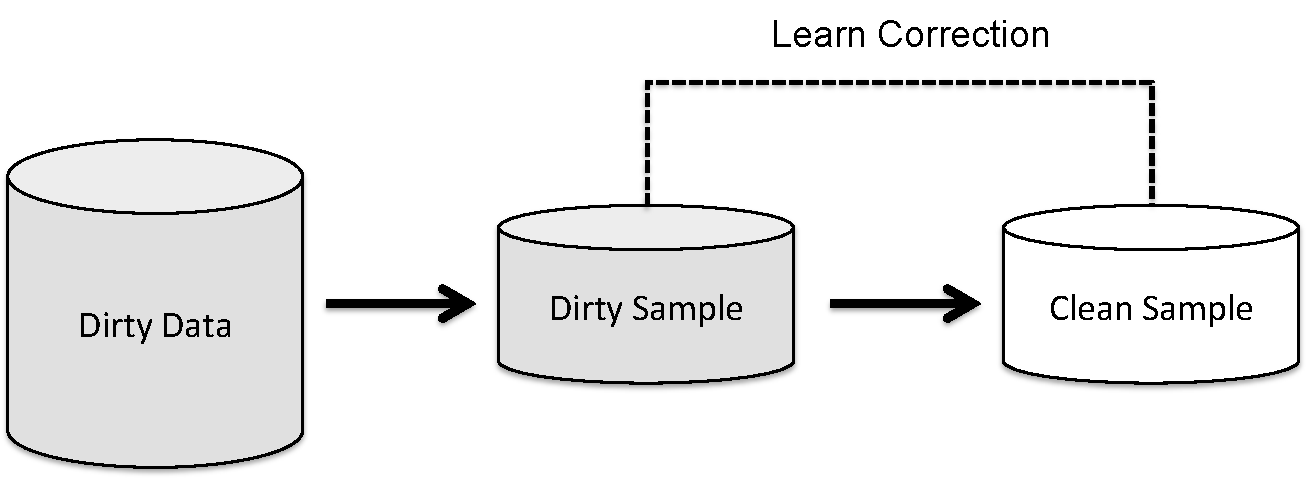
\includegraphics[scale=0.30]{figs/sys-arch2.pdf} \vspace{-.25em}
 \caption{A basic overview of SampleClean. SampleClean uses a random sample of dirty data to learn how a data cleaning algorithm affects queries on the sample. We can then derive a correction to compensate for the dirtiness.}\vspace{-1.75em}
\end{figure}

In SVC, we look at queries on stale materialized views from this perspective.
We can model a stale row in a view as dirty data.
For the data cleaning, there is some procedure (using the updates) to update this row.
For a random sample of stale data, we can apply the updates and measure how the updates change a query result and then issue a correction to acheive a result that in expectation is up-to-date.
This model gives the user access to a new tradeoff space: (1) sampling allows for reduced update costs in comparison to a full update, (2) gives better accuracy than no view maintenance.   

However, as mentioned in the introduction, this metaphor only goes so far.
Staleness can result in rows in the stale sample that are missing in the up-to-date sample.
Or, it can result in new rows in the up-to-date sample that could not possibly be in the stale sample.
In this work, we add many new contributions not considered in SampleClean: (1) we consider the effect of missing rows by using a hashing-based lineage technique, (2) we generalize our sample procedure to sample from derived relations not just the base relation as in SampleClean, (3) we explicitly consider the effects of outliers on sampling, (4) we extend the work to handle \textbf{SELECT} queries, and (5) we explore optimality of NormalizedSC.

\subsection{The Data Cleaning: Incremental Maintenance}\label{subsec-inc}
Incremental maintenance of materialized views in multiset algebras has been well studied; see \cite{chirkova2011materialized} for a survey of the approaches. 
At a high-level, almost all incremental maintenance algorithms consist of the following steps: for each leaf (relation) of the query tree of $S_{def}$ propagate $\Delta$ and $\nabla$ up the tree using composibility rules of delta relations, derive a \emph{change propagation formula} for $S$ in terms of deltas of subexpressions, and join this formula with the view to apply the changes. 
These rules are described in detail in \cite{DBLP:journals/vldb/KochAKNNLS14, DBLP:conf/pods/Koch10}.

However, even for the set of operators defined in the earlier section, there are some views for which full incremental maintenance is not possible and subexpressions have to recomputed. Consider the relation R(employeeid,country,salary) and view $S$ that calculates the \maxfunc salary of employees grouped by country. Under only insertions $\Delta R$, it is clear that the view can be maintained incrementally. 
However, if we allow deletions $\nabla R$ then it is unclear how to update a view if an employee with a maximal salary is deleted since we do not know the salary of the next highest employee. 

In cases like this, some recomputation is inevitable.
However, it turns out that SVC is general enough to handle both views that can be fully incrementally maintained and views that require partial or full recomputation.
In short, we say there is a \emph{maintenance strategy} $\mathcal{M}$ which is a relational expression that is a function of the database $\mathcal{D}$ and all the delta relations $\{\Delta R_i\} \cup \{\nabla R_i\}$ that updates the view.
SVC takes the query tree of $\mathcal{M}$ as input and outputs a sampling plan and a query correction plan (Section ??).

\subsection{Why Materialized Views Go Stale}
The algebraic analysis of incremental maintenance informs us which views can be incrementally maintained.
However, there are many practical considerations of excuting these operations in real database systems and it may not always be feasible to immediately apply updates.
For example, in distributed systems record-at-a-time maintenance may be excessively affected by overheads and batching updates together can allows for amortization.
In other systems, such as Apache Spark, the immutability of data structures means that updates can sometimes incur overheads on the order of magnitude of recomputation (see experiments ??).
Finally, immediate scheduling of maintenance can place a bottleneck on updates to the base table which may result in degraded performance or worse having to drop updates to cope with load.

The main problem is that while immediate incremental maintenance has many advantages, the particulars of the database system and available resources often dictate how updates are propagated.
To address these challenges, deferred maintenance is an alternative solution.
The main insight of deferral is to avoid maintaining the view immediately and to schedule an update at a more convenient time either in a pre-set way or adaptively.
In deferred maintenance approaches, the user often accepts some degree of staleness for additional flexibility in scheduling.
For example, views can be updated at night when the system can use more resources to process the updates without affecting a critical application.
However, this also means that during the day the materialized view becomes increasingly stale as it was computed the night before.

These costs can also be deferred to query execution time.
In particular, we highlight a technique called lazy maintenance which applies updates to the view only when a user's query requires a row \cite{zhou2007lazy}.
While always fresh, both lazy maintenance and immediate maintenance hit a bottleneck when there are rapid updates, and this results increasingly degraded performance if a user wants to query a view.
The alternative is potentially unbounded staleness between maintenance cycles with deferred maintenance.
SVC addresses this problem from a new perspective, namely, can we accept some degree of bounded inaccuracy for increased performance.

\subsection{Relationship to SAQP}
Estimating the results of aggregate queries from samples has been
well studied in a field called Sample-based Approximate Query Processing
(SAQP) \cite{OlkenR86,AgarwalMPMMS13}.
Our approach differs from SAQP as we use a sample to correct a query rather than directly estimating the query result.
The SAQP approach to this problem, would be to
estimate the result directly from the maintained sample \cite{joshi2008materialized}.
We found that estimating
a correction and leveraging an existing deterministic result led
to lower variance results on real datasets (see Section \ref{exp}). 




